\section{Base serial y tamaño de bloque}
\label{sec:base_serial}

Ejecutamos 10 repeticiones para cada tamaño de bloque $n$ con $N=2048$ y tomamos el promedio.\footnote{Compilamos con \texttt{g++ -O3 -march=native -fopenmp serial.cpp}, aunque el programa no usa OpenMP.}

\begin{figure}[htbp]
  \centering
  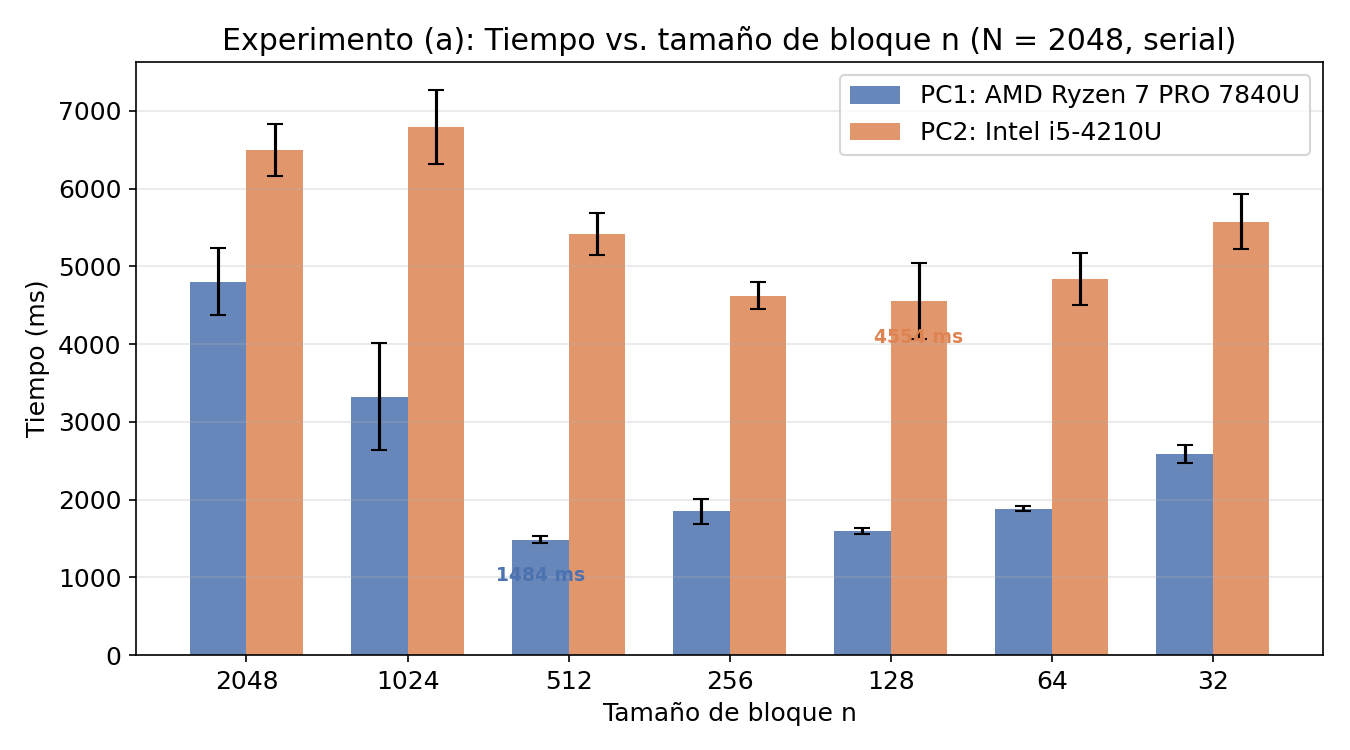
\includegraphics[width=0.9\textwidth]{A/exp_a_tiempos.png}
  \caption{Tiempo versus tamaño de bloque ($n$).}
  \label{fig:exp_a_tiempos}
\end{figure}

El parámetro $n$ controla el tamaño de los bloques en los casos base de la recursión; es decir, la matriz original se divide hasta llegar a submatrices de $n \times n$, generando un total de $(N/n)^2$ hojas donde se ejecuta la multiplicación y luego se suman los resultados. Así, el comportamiento de los tiempos forma una curva en U debido a dos factores: para $n$ grande, los bloques no caben en la memoria caché causando muchos \emph{cache misses}; y para $n$ pequeño, la cantidad de subproblemas y el \emph{overhead} de la subdivisión crecen excesivamente (por ejemplo, con $n=32$ hay 4096 hojas y 6 niveles de profundidad).

Dado lo anterior, los valores óptimos ($n=512$ en PC1 y $n=128$ en PC2) coinciden exactamente con los tamaños de bloque cuyo \emph{working set} cabe razonablemente en la caché L2 de cada procesador.\footnote{El tamaño de estas es: 1 MiB/core en el Ryzen, 256 KiB/core en el i5.}
